\section{Methodology} \label{tex:methodology}
Overall the methods examined in this thesis can be divided into two parts; namely those trying to decompose the input into a NN, and those decomposing the weights of a pre-trained NN with subsequent fine-tuning. In the following, the methods used within each of these parts will be discussed in detail. The Python library \textit{PyTorch}\cite{pytorch} will be used to implement and train all NN architectures, while all decomposition estimation will be executed using the Python library \textit{TensorLy}\cite{tensorly}. PyTorch provides a very popular application programming interface (API) for machine learning and tensor computing, which is easily accelerated using the graphics processing unit (GPU). TensorLy provides an API for tensor methods including the different decomposition methods described in \autoref{tex:decomp_methods}. TensorLy is also compatible with different back-ends\footnote{The back-end is the Python library that is responsible for low-level calculation and specification of the tensors. Typically \textit{NumPy}\cite{numpy} or \textit{PyTorch}\cite{pytorch}}, making it easy to combine with PyTorch. The algorithms used for estimating the decompositions in \textit{TensorLy} are given in \autoref{app:DecompEstimation}. 

\subsection{Decomposing the Input}
In reality, tampering with data that is going to be learned is data preprocessing, hence decomposing the input is just a form of this. Data preprocessing is a vital part of almost all ML, because structured data of high quality is simply much easier to learn and to work with. Put in another way: "Garbage in, garbage out". In addition knowledge of the structure and the variance of the data often ease the algorithm development process. The decomposition algorithms seems appropriate for this task due to their ability to exploit the structure of the data.

The Tucker decomposition is believed to be suitable for data compression tasks \cite{Mørup2011}, which is why it seems natural to apply this method to the data before feeding it in to and training the NN. The purpose is to let the decomposition do some of the learning beforehand by exploiting the variance in the data. The Tucker-decomposition is flexible since it allows for decomposition of only a subset of the dimensions\footnote{This is also called a \textit{partial} Tucker decomposition}, and because it allows for specification of ranks for each dimension individually. Since the ranks correspond to the degree of flexibility, it is easy to choose how flexible the decomposition should be along each dimension. The rank would increase with the level of desired detail. This means that if the goal of the algorithm is to differentiate a small set of features, the rank would also be kept small along the relevant dimension.

Since the observations in each the given data sets can be stacked to form a 4 (MNIST) or 5 (THETIS) dimensional tensor, it is fairly straight forward to apply the Tucker decomposition. The algorithm discussed below will only cover the MNIST data set, since the expansion to videos is trivial (one more dimension). For $N$ MNIST observations, the stacked tensor $\tensor{X}$ of size $(N \times 1 \times 28 \times 28)$ will be reshaped to $(N\times 28 \times 28)$ due to the single input channel. The decomposition of the now 3rd order tensor becomes:
\begin{equation}
    \tensor{X}^{N\times 28 \times 28} \ \approx \  \tensor{G}^{L\times J \times K} \times_1 \bs{A}^{N\times L} \times_2 \bs{B}^{28 \times J} \times_3 \bs{C}^{28 \times K}
\end{equation}
Where $L, J$ and $K$ corresponds to the ranks in each of the dimensions. Here $\tensor{G}$ is the core of the decomposition, $\bs{A}$ corresponds to the loading matrix along the between-sample dimension, while $\bs{B}$ and $\bs{C}$ correspond to the loading matrices in each of the spatial dimensions. Since the goal is to learn the differences between the different classes (digits) in the data set, only the between-sample dimension will be decomposed. The so-called Tucker-1 decomposition of the first dimension is given by:
\begin{align}
    \tensor{X}^{N\times 28 \times 28} \ &\approx \  \tensor{G}^{L\times 28 \times 28} \times_1 \bs{A}^{N\times L} \times_2 \bs{I}^{28 \times 28} \times_3 \bs{I}^{28 \times 28} \\
    &\approx \tensor{G}^{L\times 28 \times 28} \times_1 \bs{A}^{N\times L}
\end{align}
This is equivalent to SVD using the unfolded representation with respect to the first dimension:
\begin{equation}
    \bs{X}_{(1)} = \bs{A} \bs{G}_{(1)}
    \label{eq:tuckerMNISTinput}
\end{equation}
Now the loading matrix $\bs{A}$ holds information about what differentiates the different samples using only $L$ features. These features will be used as the input into a very simple ANN, potentially lowering the number of input nodes dramatically if $L$ is kept small. The algorithm is illustrated in \autoref{fig:illustrationinputdecomp}.

In this project experiments will be made with different architectures for the simple ANN (i.e. number of hidden neurons in the hidden layer(s) $H$), along with different values of the rank $L$. The results will be provided and discussed in terms of the trade-off between computational speed and accuracy.

\begin{figure}
    \centering
    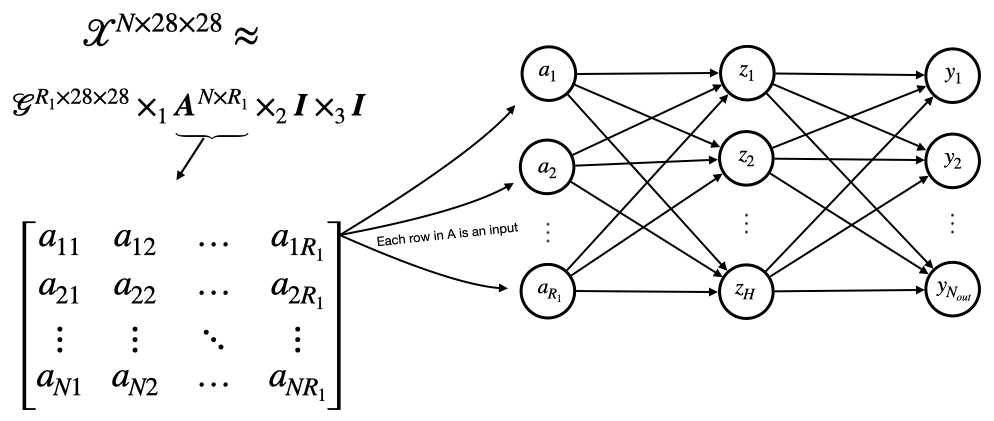
\includegraphics[width=\linewidth]{Pics/05_methodology/input_decomp_illustration.png}
    \captionsetup{width=.95\linewidth}
    \caption{Illustration of the algorithm that decomposes the input into the NN. The stacked data tensor will be decomposed along the between-sample dimension resulting in a loading matrix $\bs{A}$ which holds $L$ values for each observation, which will then be used as input into a simple ANN}
    \label{fig:illustrationinputdecomp}
\end{figure}

\subsubsection{Estimating the loadings for the testing data}
Since the testing data cannot be decomposed along with the training data, the loading matrix for the testing data will be estimated assuming the same core as for the training data. This way the decomposition is also a part of the training. Based on \eqref{eq:tuckerMNISTinput} the loading matrix for the test set can be estimated by multiplying with the pseudo-inverse of the matricized core:
\begin{equation}
    \bs{A}_{test} \approx {\bs{X}_{test}}_{(1)} \bs{G}_{(1)}^{\ \dagger}
\end{equation}
The two matrices $\bs{A}$ and $\bs{A}_{test}$ will be given as the input to the ANN as the training data and the validation/testing data respectively.


%%%%%%%%%%%%%%%%%%%%%%%%%%%%%%%%%%%%%%%%%%%%%%%%%%%%%%%%%%%%%%%%%%%%%%%%%%%%%%%%%%%%    
%%        Decomposing Pre-Trained Network    %%%%%%%%%%%%%%%%%%%%%%%%%%%%%%%%%%%%%%%
%%%%%%%%%%%%%%%%%%%%%%%%%%%%%%%%%%%%%%%%%%%%%%%%%%%%%%%%%%%%%%%%%%%%%%%%%%%%%%%%%%%%

\subsection{Decomposing a Pre-Trained Network Using Tucker Decomposition}
Using this approach is relatively easy to justify which is properly the reason why all the methods discussed in \autoref{tex:previous_work} use this approach. Pre-training a network makes it easier to ensure a network that works well, also because the training is often performed on powerful computers which allows for more complex networks. After the training is concluded the network is only decomposed to optimise the evaluation time in order to make it useful on platforms with less computation power. As discussed in \autoref{tex:previous_work} there are multiple approaches for this, but especially the methods using Tucker-decomposition and BTD seamed to be performing well and relatively straight-forward to implement and fine-tune.
The method used in this project builds on the work done by Kim et al. in \cite{Kim2016}, which is briefly discussed in \autoref{tex:sub_entire_network}.  Similar to the work done by Kim et al., Tucker-1 or Tucker-2 will be used for specific layers through the network. The advantage of using Tucker-decompositions is that they can be applied to each of the layers in the network, compressing everything at once before fine-tuning the whole network. In the following the methods of decomposing and changing the architecture of the layers of the network will be discussed. Due to the dissimilarities of the linear vs. the convolutional layer, each of these decompositions will be implemented individually for each type of layer. In the end, the full algorithm for compressing a whole network will be given.

\subsubsection{The linear / dense layer}
As explained in \autoref{tex:theory_NN} the dense layer with $N_{in}$ input neurons and $N_{out}$ output neurons in simply a matrix-vector product:
\begin{equation}
    \bs{y}^{N_{out}} = \bs{W}^{N_{out}\times N_{in}}\bs{x}^{N_in} + \bs{b}^{N_{out}}
    \label{eq:linearLayerTransformWOdecomp}
\end{equation}
Where $\bs{x}$ is the input, $\bs{y}$ is the input, $\bs{b}$ is the bias vector, and $\bs{W}$ is the weight matrix. The weight matrix is potentially big resulting in many parameters and high calculation time. The idea of the decomposed linear layer is to decompose the weight tensor into a set of smaller matrices that can be multiplied sequentially resulting in higher efficiency. The Tucker-1 and Tucker-2 decompositions of the weight matrix are given as:
\begin{align}
\texttt{Tucker-1}&: \quad \bs{W} \approx \bs{G} \times_1 \bs{A} \times_2 \bs{I} = \bs{A}\bs{G} \qquad \text{OR} \qquad \bs{W} \approx \bs{G} \times_1 \bs{I} \times_2 \bs{B} = \bs{G}\bs{B}^\top \\
\texttt{Tucker-2}&: \quad \bs{W} \approx \bs{G} \times_1 \bs{A} \times_2 \bs{B} = \bs{A}\bs{G}\bs{B}^\top 
\end{align}
Here $\bs{I}$ is the identity matrix and the core tensor $\bs{G}$ is a matrix due to the weight matrix $\bs{W}$ only having 2 dimensions. The type of Tucker-1 decomposition is chosen based on which dimension is to be decomposed.\footnote{Dense layers often go from many inputs to a fewer outputs why the input dimension might be more desirable to compress.} Inserting the decomposition of $\bs{W}$ in the linear transform \eqref{eq:linearLayerTransformWOdecomp} yields:
\begin{align}
     \bs{y}^{N_{out}} &\approx \bs{A}^{N_{out}\times R_A} \bs{G}^{R_A\times N_{in}} \bs{x}^{N_{in}} + \bs{b}^{N_{out}} \\
    \texttt{Tucker-1}: \qquad \quad \ \ &\text{OR} \nonumber \\
    \bs{y}^{N_{out}} &\approx \bs{G}^{N_{out}\times R_B} \bs{B}^{\top \  R_B\times N_{in}}\bs{x}^{N_{in}} + \bs{b}^{N_{out}} \\
    &\quad \nonumber \\
    \texttt{Tucker-2}: \quad \bs{y}^{N_{out}} &\approx \bs{A}^{N_{out}\times R_A} \bs{G}^{R_A\times N_{in}} \bs{B}^{\top  R_B\times N_{in}}\bs{x}^{N_{in}} + \bs{b}^{N_{out}}
\end{align}
Now looking at the number of multiplications needed to do each of the products from right to left gives the values in \autoref{tab:numberOfMultiplicationsLinearLayer}. For instance using the Tucker-1 compression uses $N_{in}R + RN_{out}=R(N_{out}+N_{in})$ multiplications to do the matrix-product. The table also shows the restrictions on the ranks to have less multiplications than the uncompressed version, hence to be more efficient.
\begin{table}
    \centering
    \captionsetup{width=.9\linewidth}
    \caption{The number of multiplications needed to do the matrix-vector product in the linear layer \eqref{eq:linearLayerTransformWOdecomp} with the weight matrix decomposed using Tucker-1 and Tucker-2. The matrix product is assumed to be calculated from right to left.}
    \begin{tabular}{l|c|c}
        \textbf{Method} & \textbf{\# Multiplications} & \textbf{Faster when:} \\ \hline
        Uncrompressed & $N_{out} N_{in}$ & - \\
        Tucker-1 & $R(N_{in} + N_{out})$ & $R < \frac{N_{out}N_{in}}{N_{out} + N_{in}}$\\
        Tucker-2 & $N_{in}R_B + R_BR_A + R_AN_{out}$ & $(N_{in}+R_A)(N_{out}+R_B) < 2 N_{in}N_{out}$
    \end{tabular}
    \label{tab:numberOfMultiplicationsLinearLayer}
\end{table}

What also makes this decomposition smart is that the sequence of matrix multiplications can be achieved by a sequence of 2 or 3 linear layers, where the loadings from the decomposition can be directly used as weights. This makes it straight-forward to adapt the layer into a decomposed version and to fine-tune. The concept is illustrated in \autoref{fig:diffNNlinearLayer}. The biases from the original layer will be added only to the last layer in the sequence of the decomposed version and they will not be modified in any way.
\begin{figure}
    \centering
    \begin{subfigure}{0.35\linewidth}
        \centering
        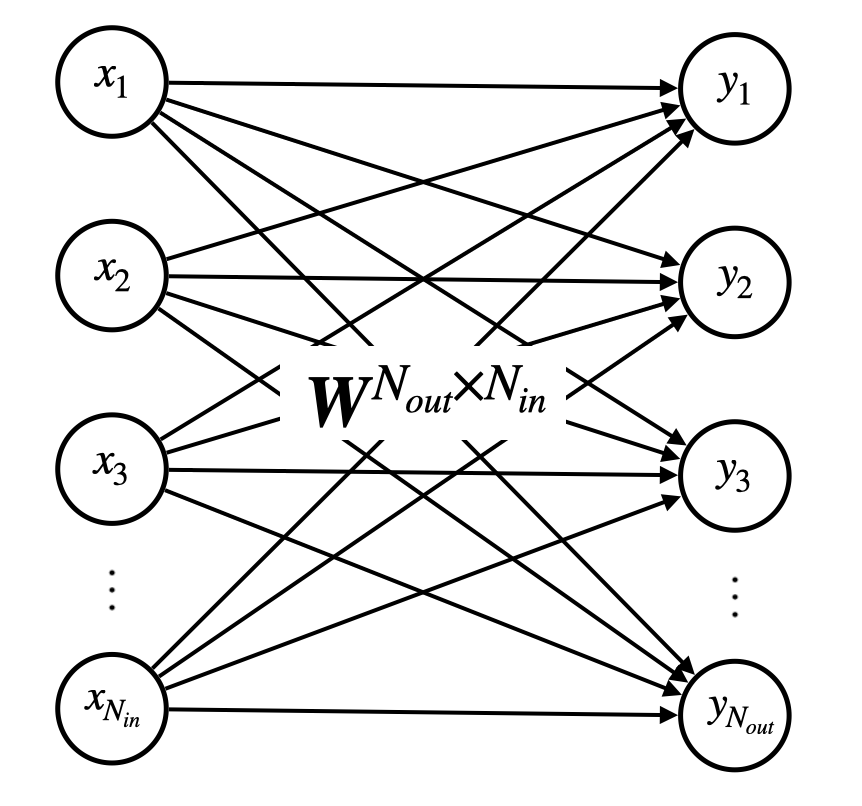
\includegraphics[width=\linewidth]{Pics/05_methodology/NNlinearLayer.png}
        \caption{Original linear layer}
    \end{subfigure}
    \begin{subfigure}{\linewidth}
        \centering
        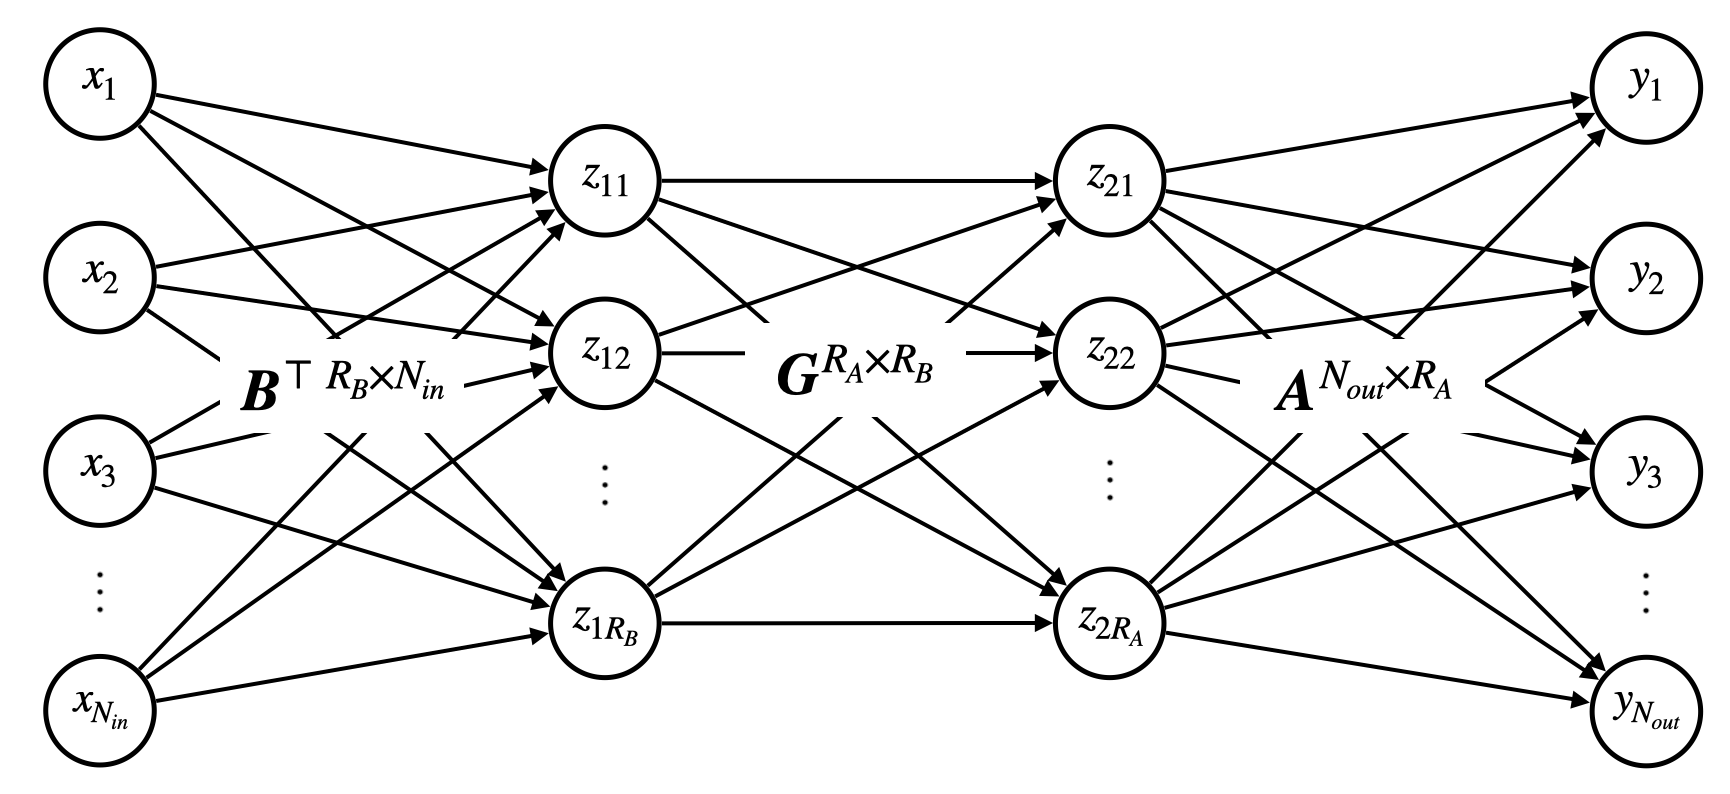
\includegraphics[width=.7\linewidth]{Pics/05_methodology/NNdecompLinearLayer.png}
        \caption{Sequence of linear layers resulting after decomposing $\bs{W}$}
    \end{subfigure}
    \captionsetup{width=.9\linewidth}
    \caption{Illustration of the difference between the original linear layer and the decomposed sequence of linear layers. The matrices $\bs{A}, \bs{B}$ and $\bs{G}$ are the resulting loading matrices and core respectively after decomposing the original weight matrix $\bs{W}$. The biases from the original layer will be added only to the last layer in the decomposed sequence.}
    \label{fig:diffNNlinearLayer}
\end{figure}

\subsubsection{The convolutional layer}
As explained in \autoref{tex:theory_NN} a convolution corresponds to calculating the result of applying a number of filters to every part of the input picture or video in space (and time). Applying the Tucker-decomposition to a convolutional layer implies turning it into a sequence of 3 (Tucker-2) or 2 (Tucker-1) smaller, less computational convolutions. The following method will only be discussed for videos, since the calculations are almost identical for lower dimensions. See \cite{Kim2016} for these, which the following derivation is based upon.

\paragraph{Tucker-2 decomposition of the convolutional kernel}
The convolution of an input tensor $\tensor{X}$ of size\footnote{Here and in the following $F$, $H$, $W$ are the number of frames, the height and the width of the video respectively. $S$ is the number of input channels.} $F\times H \times W \times S$ into an output tensor $\tensor{Y}$ of size $F'\times H' \times W' \times T$ is given by:
\begin{equation}
    \tensor{Y}(f', h', w', t) = \sum_{i=1}^{D_F} \sum_{j=1}^{D_H} \sum_{l=1}^{D_W} \sum_{s=1}^{S} \ \tensor{K}(i, j, l, s, t) \ \tensor{X}(f_i, h_j, w_l, s)
    \label{eq:3d_convolution}
\end{equation}
Where:
\begin{equation}
    f_i = \left(f' - 1\right) \Delta_F + i - P_F \qquad h_j =  \left(h' - 1\right) \Delta_H + j - P_H \qquad w_l =  \left(w' - 1\right) \Delta_W + l - P_W
\end{equation}
Where the $\Delta$s are the strides in each of the dimensions, the $P$s are the corresponding padding, and ($f'$, $h'$, $w'$, $t$) is the position in the output tensor $\tensor{Y}$. $\tensor{K}$ is the 5-dimensional convolutional kernel, i.e. the stack of 4-dimensional filters, and the $D$s are the filter sizes in each of the spatial and temporal dimensions. Now the Tucker-2 decomposition of $\tensor{K}$ in the input and output channel dimensions is expressed by:
\begin{equation}
\tensor{K}(i, j, l, s, t)=\sum_{r_{4}=1}^{R_{4}} \sum_{r_{5}=1}^{R_{5}} \tensor{C}(i, j, l, r_{4}, r_{5}) \ \boldsymbol{U}^{(4)}(s, r_{4}) \  \boldsymbol{U}^{(5)}(t, r_{5})
\end{equation}
Where $\tensor{C}$ is the core of the decomposition of size $D_F\times D_H \times D_W \times S \times T$ and the $\bs{U}$s are the loading matrices along the input and output dimensions respectively. Now substituting this expression into \eqref{eq:3d_convolution} gives:
\begin{equation}
    \tensor{Y}(f', h', w', t) = \sum_{i=1}^{D_F} \sum_{j=1}^{D_H} \sum_{l=1}^{D_W} \sum_{s=1}^{S} \sum_{r_{4}=1}^{R_{4}} \sum_{r_{5}=1}^{R_{5}} \tensor{C}(i, j, l, r_{4}, r_{5}) \ \boldsymbol{U}^{(4)}(s, r_{4}) \  \boldsymbol{U}^{(5)}(t, r_{5}) \ \tensor{X}(f_i, h_j, w_l, s)
\end{equation}
Rearranging, since not all factors depend on $s$, yields:
\begin{equation}
    \tensor{Y}(f', h', w', t) = \sum_{i=1}^{D_F} \sum_{j=1}^{D_H} \sum_{l=1}^{D_W} \sum_{r_{4}=1}^{R_{4}} \sum_{r_{5}=1}^{R_{5}} \tensor{C}(i, j, l, r_{4}, r_{5}) \ \boldsymbol{U}^{(5)}(t, r_{5}) \ \underbrace{\sum_{s=1}^{S} \boldsymbol{U}^{(4)}(s, r_{4}) \ \tensor{X}(f_i, h_j, w_l, s)}_{\large \tensor{Q}}
\end{equation}
Summing out $s$ yields an intermediate tensor $\tensor{Q}$ of size $F\times H \times W \times R_4$. Doing the same again:
\begin{equation}
    \tensor{Y}(f', h', w', t) = \sum_{i=1}^{D_F} \sum_{j=1}^{D_H} \sum_{l=1}^{D_W} \sum_{r_{4}=1}^{R_{4}} \sum_{r_{5}=1}^{R_{5}} \tensor{C}(i, j, l, r_{4}, r_{5}) \ \boldsymbol{U}^{(5)}(t, r_{5}) \  \tensor{Q} (f_i, h_j, w_l, r_4)
\end{equation}
Rearranging:
\begin{equation}
    \tensor{Y}(f', h', w', t) = \sum_{r_{5}=1}^{R_{5}} \ \boldsymbol{U}^{(5)}(t, r_{5}) \ \underbrace{\sum_{i=1}^{D_F} \sum_{j=1}^{D_H} \sum_{l=1}^{D_W} \sum_{r_{4}=1}^{R_{4}} \tensor{C}(i, j, l, r_{4}, r_{5})   \tensor{Q} (f_i, h_j, w_l, r_4)}_{\large \tensor{Q}'}
\end{equation}
Summing out everything but the output channels yields a new intermediate tensor $\tensor{Q}'$ of size $F' \times H' \times W' \times R_5$, and the convolution can now be expressed in terms of $\tensor{Q}'$:
\begin{equation}
    \tensor{Y}(f', h', w', t) = \sum_{r_{5}=1}^{R_{5}} \ \boldsymbol{U}^{(5)}(t, r_{5}) \ \tensor{Q}'(f', h', w', r_5)
\end{equation}
But now we have that the three intermediate tensors given by:
\begin{align}
    \tensor{Q}(f, h, w, r_4) &= \sum_{s=1}^{S} \boldsymbol{U}^{(4)}(s, r_{4}) \ \tensor{X}(f, h, w, s) \label{eq:Q}\\
    \tensor{Q'}(f', h', w', r_5) &= \sum_{i=1}^{D_F} \sum_{j=1}^{D_H} \sum_{l=1}^{D_W} \sum_{r_{4}=1}^{R_{4}} \tensor{C}(i, j, l, r_{4}, r_{5})   \tensor{Q} (f_i, h_j, w_l, r_4) \label{eq:Q'} \\
    \tensor{Y}(f', h', w', t) &=  \sum_{r_{5}=1}^{R_{5}} \ \boldsymbol{U}^{(5)}(t, r_{5}) \ \tensor{Q}'(f', h', w', r_5) \label{eq:Y}
\end{align}
correspond to the following sequence of simpler convolutions:
\begin{itemize}
    \item Eq. \eqref{eq:Q} - A $1\times 1$ convolution with $S$ input channels and $R_4$ output channels (the rank of the decomposition)
    \item Eq. \eqref{eq:Q'} - A $D_F \times D_H \times D_W$ convolution with $R_4$ input channels and $R_5$ output channels
    \item Eq. \eqref{eq:Y} - A $1\times 1$ convolution with $R_5$ input channels and $T$ output channels
\end{itemize}
So what this sequence is actually doing is first using the $1\times 1$ convolution to bring down the number of input channels to the 3D convolution, in order to perform the 3D convolution on a smaller set of input and output channels. In the end it uses the $1\times 1$ convolution to bring the now lower number of output channels back up to what it should be. This all results in a speed-up if the ranks are chosen to be small. Due to the challenge of illustrating a 4D tensor, the concept is illustrated in the 2D version (a picture) in \autoref{fig:tuckerDecompConv}. Like for the linear layer, the loadings of the decomposition of the kernel $\tensor{K}$ can be used directly as weights in the adapted architecture, and also the original biases will only be added to the last layer, while the other wont have biases.

\paragraph{Tucker-1 decomposition of the convolutional kernel}
In some situations it might not be beneficial to decompose both the input and the output channel dimensions, e.g. for an input image with only 3 input channels. The approach when doing the Tucker-1 decomposition is the same as for the Tucker-2 decomposition, however only one (relevant) rank is considered. This means that the resulting sequence have two smaller convolutions, and that there will be only two intermediate tensors corresponding to \eqref{eq:Q} and \eqref{eq:Q'} if the input channel dimension is to be decomposed, or \eqref{eq:Q'} and \eqref{eq:Y} for the output channel dimension. The derivations will be given for each of the dimensions in \autoref{tex:tucker1_conv_derivations}.

\subsubsection{Rank Selection}

\subsubsection{One-Shot Compression a an entire CNN Using Tucker}
Using the different algorithms for compressing a single layer in the CNN and appropriate ranks, the algorithm for compressing a whole CNN is given in \autoref{alg:one_shot_tucker}. The algorithm is basically training an appropriate network, decomposing all the layers given the methods above, and then fine-tuning the new decomposed network.

\begin{algorithm} \caption{One-Shot Tucker Compression of CNN} \label{alg:one_shot_tucker}
\begin{algorithmic}[1]
    \State $\texttt{net} \leftarrow $ define an appropriate CNN
    \State train $\texttt{net}$ using the given training data
    \State $\texttt{net\_dcmp} \leftarrow $ make a copy of $\texttt{net}$
    \For{each \textbf{convolutional} layer; $\texttt{layer}$ in $\texttt{net\_dcmp}$}
        \State $\tensor{K}_{\texttt{layer}} \leftarrow $ take out weight tensor
        \State $R_4, R_5 \leftarrow$ choose appropriate rank(s)
        \State $\tensor{G}, \ \ \bs{U}^{(4)}, \bs{U}^{(5)} \leftarrow $ Decompose $\tensor{K}_{\texttt{layer}}$ using relevant algorithm \Comment{Or just one $\bs{U}$}
        \State $\texttt{layer\_dcmp\_1} \leftarrow $ define new $1\times 1$ convolution \Comment{If applicable}
        \State $\texttt{layer\_dcmp\_2} \leftarrow $ define new 3D convolution
        \State $\texttt{layer\_dcmp\_3} \leftarrow $ define new $1\times 1$ convolution \Comment{If applicable}
        \State $\tensor{K}_{\texttt{layer\_dcmp\_1}} \leftarrow \bs{U}^{(4)}$ \Comment{If applicable}
        \State $\tensor{K}_{\texttt{layer\_dcmp\_2}} \leftarrow \tensor{G}$
        \State $\tensor{K}_{\texttt{layer\_dcmp\_3}} \leftarrow \bs{U}^{(5)}$ \Comment{If applicable}
        \State $\bs{b}_{\texttt{layer\_dcmp\_3}} \leftarrow \bs{b}_{\texttt{layer}}$ add the bias to the last layer \Comment{Or in the line above}
        \State $\texttt{layer} \leftarrow \texttt{sequence}(\texttt{layer\_dcmp\_1}, \  \texttt{layer\_dcmp\_2}, \ \texttt{layer\_dcmp\_3})$
    \EndFor
    \For{each \textbf{linear} layer; $\texttt{layer}$ in $\texttt{net\_dcmp}$}
        \State $\bs{W}_{\texttt{layer}} \leftarrow $ take out weight matrix of size $N_{out} \times N_{in}$
        \State $R_A, R_B \leftarrow $ choose appropriate rank(s)
        \State $\bs{G}, \bs{A}, \bs{B} \leftarrow $ decompose $\bs{W}_{\texttt{layer}}$ using relevant algorithm \Comment{Or just $\bs{A}$ or $\bs{B}$}
        \State $\texttt{layer\_dcmp\_1} \leftarrow $ define new $R_B \times N_{in}$ linear layer \Comment{If applicable}
        \State $\texttt{layer\_dcmp\_2} \leftarrow $ define new $R_A \times R_B$ linear layer \Comment{Or $R_B\times N_{in}$ or $N_{out}\times R_A$}
        \State $\texttt{layer\_dcmp\_3} \leftarrow $ define new $N_{out} \times R_A$ linear layer \Comment{If applicable}
        \State $\bs{W}_{\texttt{layer\_dcmp\_1}} \leftarrow \bs{B}$ \Comment{If applicable}
        \State $\bs{W}_{\texttt{layer\_dcmp\_2}} \leftarrow \bs{G}$
        \State $\bs{W}_{\texttt{layer\_dcmp\_3}} \leftarrow \bs{A}$ \Comment{If applicable}
        \State $\bs{b}_{\texttt{layer\_dcmp\_3}} \leftarrow \bs{b}_{\texttt{layer}}$ add the bias to the last layer \Comment{Or in the line above}
        \State $\texttt{layer} \leftarrow \texttt{sequence}(\texttt{layer\_dcmp\_1}, \ \texttt{layer\_dcmp\_2}, \ \texttt{layer\_dcmp\_3})$
    \EndFor
    \State train $\texttt{net\_dcmp}$ using the given training data \Comment{fine-tuning}
\end{algorithmic}
\end{algorithm}